%-----------------------------------------------------------------------------%
\chapter{\babDua}
\label{bab:2}
%-----------------------------------------------------------------------------%
\todo{
	Bab ini, biasanya namanya adalah "Studi Literatur" atau "Tinjauan Pustaka".
	Akan tetapi, beberapa fakultas atau dosen pembimbing meminta Bab 2 untuk dinamakan lain, seperti "Kerangka Berpikir".
}

Untuk memulai penelitian, dibutuhkan kerangka berpikir yang sesuai untuk permasalahan yang ingin dipecahkan.
Untuk membentuk kerangka berpikir yang sesuai, perlu dikaitkan dengan hasil studi literatur yang telah dilakukan.
Oleh karena itu, pada bab ini, akan dijelaskan hasil studi literatur yang telah dilakukan yang telah dikaitan dengan kerangka kerja untuk penelitian ini.


%-----------------------------------------------------------------------------%
\section{Apa itu \latex?}
\label{sec:latex}
%-----------------------------------------------------------------------------%

%-----------------------------------------------------------------------------%
\subsection{\latex~Secara Singkat}
\label{sec:latexBrief}
%-----------------------------------------------------------------------------%
Berdasarkan \cite{latex:intro}: \\
\begin{tabular}{| p{14cm} |}
	\hline
	\gls{latex} is a family of programs designed to produce publication-quality typeset documents.
	It is particularly strong when working with mathematical symbols. \\
	The history of \gls{latex} begins with a program called TEX.
	In 1978, a computer scientist by the name of Donald Knuth grew frustrated with the mistakes that his publishers made in typesetting his work.
	He decided to create a typesetting program that everyone could easily use to typeset documents, particularly those that include formulae, and made it freely available.
	The result is TEX. \\
	Knuth's product is an immensely powerful program, but one that does focus very much on small details.
	A mathematician and computer scientist by the name of Leslie Lamport wrote a variant of TEX called \gls{latex} that focuses on document structure rather than such details. \\
	\hline
\end{tabular}

\vspace*{0.2cm}

Dokumen \gls{latex}~sangat mudah, seperti halnya membuat dokumen teks biasa.
Ada beberapa perintah yang diawali dengan tanda '\bslash'.
Seperti perintah \code{\bslash\bslash}~yang digunakan untuk memberi baris baru.
Perintah tersebut juga sama dengan perintah \code{\bslash{}newline}.
Pada bagian ini akan sedikit dijelaskan cara manipulasi teks dan perintah-perintah \gls{latex}~yang mungkin akan sering digunakan.
Jika ingin belajar hal-hal dasar mengenai \gls{latex}, silakan kunjungi:

\begin{itemize}
	\item \url{http://frodo.elon.edu/tutorial/tutorial/}, atau
	\item \url{http://www.maths.tcd.ie/~dwilkins/LaTeXPrimer/}
\end{itemize}

%-----------------------------------------------------------------------------%
\subsection{\latex~Kompiler dan IDE}
\label{sec:latexCompiler}
%-----------------------------------------------------------------------------%
Untuk menggunakan \gls{latex}~(pada konteks hanya sebagai pengguna), tidak perlu banyak tahu mengenai hal-hal didalamnya.
Dengan menggunakan \f{Integrated Development Environment} (IDE), penggunaan \gls{latex}~akan serupa dengan pembuatan dokumen secara visual, layaknya OpenOffice Writer atau Microsoft Word.
Orang-orang yang menggunakan \gls{latex}~relatif lebih teliti dan terstruktur mengenai cara penulisan yang dia gunakan, karena \gls{latex}~memaksa untuk seperti itu.

Untuk mencoba \gls{latex}, diperlukan kompiler dan IDE.
Bagi pengguna Microsoft Windows dan Mac OS, instalasi kompiler \gls{latex}~dapat menggunakan MikTeX (\url{https://miktex.org/download}).
Bagi pengguna Linux, instalasi kompiler \gls{latex}~dapat menggunakan Texlive ( \url{http://www.tug.org/texlive/}).
Distro-distro \f{mainstream} di Linux seperti Ubuntu biasanya telah menyediakan \f{package} \code{texlive} melalui \f{package manager}.
Apabila ingin melakukan instalasi Texlive melalui \f{package manager}, lakukan instalasi package \code{texlive-full} atau setidaknya \code{texlive-science} agar prasyarat \f{template} ini tersedia secara lengkap.

Beberapa text editor atau IDE yang dapat digunakan adalah sebagai berikut:
\begin{itemize}
	\item \underline{\href{https://www.texstudio.org/}{TeXstudio}} (direkomendasikan),
	\item TeXWorks (biasanya bawaan dari \underline{\href{https://miktex.org/download}{MikTeX}}),
	\item \underline{\href{http://www.xm1math.net/texmaker/}{Texmaker}}, atau
	\item Microsoft Visual Studio Code, dengan \f{plugin} \underline{\href{https://marketplace.visualstudio.com/items?itemName=James-Yu.latex-workshop}{\gls{latex} Workshop}}.
	Untuk menggunakan \f{plugin} tersebut, diperlukan instalasi MikTeX dan Perl.
	Alternatif lain untuk persyaratan tersebut adalah menggunakan \f{plugin} Remote - WSL jika memiliki distro Windows Subsystem for Linux (WSL) 2 yang sudah terpasang \code{texlive}.
\end{itemize}


%-----------------------------------------------------------------------------%
\section{\f{Formatting} Teks Dasar}
\label{sec:latexBasicFormatting}
%-----------------------------------------------------------------------------%
Hal pertama yang mungkin ditanyakan adalah bagaimana membuat huruf tercetak tebal, miring, atau memiliki garis bawah.
Pada Texmaker, Anda bisa melakukan hal ini seperti halnya saat mengubah dokumen dengan OO Writer.
Namun jika tetap masih tertarik dengan cara lain, ini dia:

\begin{itemize}
	\item \bo{Bold} \\
	Gunakan perintah \code{\bslash{}textbf$\lbrace\rbrace$} atau
	\code{\bslash{}bo$\lbrace\rbrace$}.\\
	Contoh: \textbf{Contoh hasil tulisan} atau \bo{Contoh hasil tulisan}.
	\item \f{Italic} \\
	Gunakan perintah \code{\bslash{}textit$\lbrace\rbrace$} atau
	\code{\bslash{}f$\lbrace\rbrace$}.\\
	Contoh: \textit{Contoh hasil tulisan} atau \f{Contoh hasil tulisan}.
	\item \underline{Underline} \\
	Gunakan perintah \code{\bslash{}underline$\lbrace\rbrace$}.\\
	Contoh: \underline{Contoh hasil tulisan}.
	\item $\overline{Overline}$ \\
	Gunakan perintah \code{\$\bslash{}overline\$}.\\
	Contoh: $\overline{Contoh~hasil~tulisan}$.
	\item $^{superscript}$ \\
	Gunakan perintah \code{\$\bslash{}$\lbrace\rbrace$\$}.\\
	Contoh: $^{Contoh~hasil~tulisan}$.
	\item $_{subscript}$ \\
	Gunakan perintah \code{\$\bslash{}\_$\lbrace\rbrace$\$}.\\
	Contoh: $_{Contoh~hasil~tulisan}$.
\end{itemize}

% v2.2.1: tutorial dipindah dari Bab 3 ke Bab 2
Ada beberapa hal lain yang bisa digunakan.
\begin{itemize}
	\item Kombinasi \bo{Bold} dan \f{Italic}: \\
	Gunakan perintah \code{\bslash{}bi$\lbrace\rbrace$}. \\
	Contoh: \bi{Contoh hasil tulisan}.
	\item Menebalkan teks formula matematis: \\
	Gunakan perintah \code{\bslash{}m$\lbrace\rbrace$}. \\
	Contoh: \m{\alpha~\beta}
	\item Menebalkan teks formula matematis, sekaligus meletakkannya di tengah: \\
	Gunakan perintah \code{\bslash{}mc$\lbrace\rbrace$}. \\
	Contoh: \mc{\alpha~\beta}
	\item Menggunakan \f{monospaced font} untuk kode:
	Gunakan perintah \code{\bslash{}texttt$\lbrace\rbrace$} atau \code{\bslash{}code$\lbrace\rbrace$}. \\
	Contoh: \texttt{Contoh hasil tulisan} atau \code{Contoh hasil tulisan}.
\end{itemize}

Perintah \code{\bslash{}f}, \code{\bslash{}bo}, \code{\bslash{}bi}, \code{\bslash{}m}, \code{\bslash{}mc},
dan \code{\bslash{}code} hanya dapat digunakan jika package \code{\_internals/uithesis} digunakan.

%-----------------------------------------------------------------------------%
\section{Memasukan Gambar}
\label{sec:latexImage}
%-----------------------------------------------------------------------------%
Setiap gambar dapat diberikan caption dan diberikan label. Label dapat digunakan untuk menunjuk gambar tertentu.
Jika posisi gambar berubah, maka nomor gambar juga akan diubah secara otomatis.
Begitu juga dengan seluruh referensi yang menunjuk pada gambar tersebut.
Contoh sederhana adalah \pic~\ref{fig:testGambar}, yang bisa dibuat dengan menggunakan \lst~\ref{code:latexImage}.
Harap diingat pada aturan Tugas Akhir UI, caption harus selalu \b{diletakkan di bawah gambar}.

\lstinputlisting[language={[latex]tex}, caption=Contoh penggunaan gambar, label=code:latexImage]{assets/codes/tutorial/2-basicFigure.tex}

Berikut adalah penjelasan dari \lst~\ref{code:latexImage}:
\begin{itemize}
	\item Baris ke-2: \code{\bslash{}centering} digunakan untuk membuat gambar berada di tengah.
	\item Baris ke-3 dan 4: \code{\bslash{}includegraphics} digunakan untuk memasukkan gambar. \\
	\code{width=0.25\bslash{}textwidth} digunakan untuk mengatur lebar gambar sebesar 25\% dari lebar teks (dari ujung marjin kiri ke ujung marjin kanan).
	\item Baris ke-5: \code{\bslash{}caption} digunakan untuk memberikan \f{caption} pada gambar.
	\f{Caption} tersebut diletakkan setelah \code{includegraphics} agar \f{caption} berada di bawah gambar.
	\item Baris ke-6: \code{\bslash{}label} digunakan untuk memberikan label pada gambar.
	Label ini bisa digunakan di suatu paragraf untuk merujuk pada gambar tersebut,
	dengan cara menuliskan \code{\bslash{}ref\{label\}} pada paragraf.
\end{itemize}

\begin{figure}
	\centering
	
\includegraphics[width=0.25\textwidth]
	{assets/pics/makara_kuning.png}
	\caption{Makara Universitas Indonesia}
	\label{fig:testGambar}
\end{figure}


Anda juga bisa memasukkan sitasi atau URL sumber gambar, jika gambar tersebut bukan Anda sendiri yang membuatnya.
Contoh sederhana adalah \pic~\ref{fig:testGambarBersumber}, yang bisa dibuat dengan menggunakan \lst~\ref{code:latexImageSource}.

\lstinputlisting[language={[latex]tex}, caption=Contoh penggunaan gambar bersumber, label=code:latexImageSource]{assets/codes/tutorial/2-sourcedFigure.tex}

Pada baris ke-5, \code{\bslash{}captionsource} digunakan untuk memberikan caption dan sumber gambar.
Dalam kasus ini, sumber gambar merupakan sebuah URL, sehingga ditandai dengan perintah \code{\bslash{}url\{\}}.
Jika sumber gambar merupakan sebuah buku, jurnal, atau dokumen, maka bisa dilakukan sitasi menggunakan perintah \code{\bslash{}cite\{\}}.
Contoh: \code{\bslash{}captionsource\{Sesuatu\}\{\bslash{}cite\{latex:intro\}\}}.

\begin{figure}
	\centering
	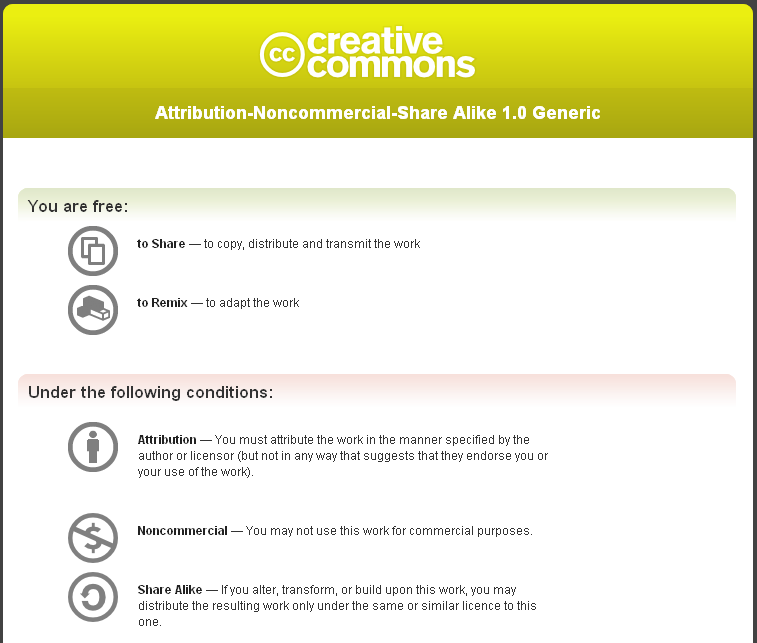
\includegraphics[width=0.50\textwidth]
	{assets/pics/creative_commons.png}
	\captionsource{\license.}{{\url{https://creativecommons.org/licenses/by-nc-sa/1.0/}}}
	\label{fig:testGambarBersumber}
\end{figure}



%-----------------------------------------------------------------------------%
\section{Membuat Tabel}
\label{sec:latexTable}
%-----------------------------------------------------------------------------%
Tabel pada \gls{latex} dapat dibuat secara visual dengan bantuan \f{website} seperti \url{https://www.tablesgenerator.com/}.
Dengan menggunakan \textit{website} ini, maka pembuatan tabel akan menjadi lebih mudah.
\textit{User interface} dari \f{website} dapat dilihat pada Gambar \ref{fig:tablesgenerator}.

\begin{figure}
	\centering
	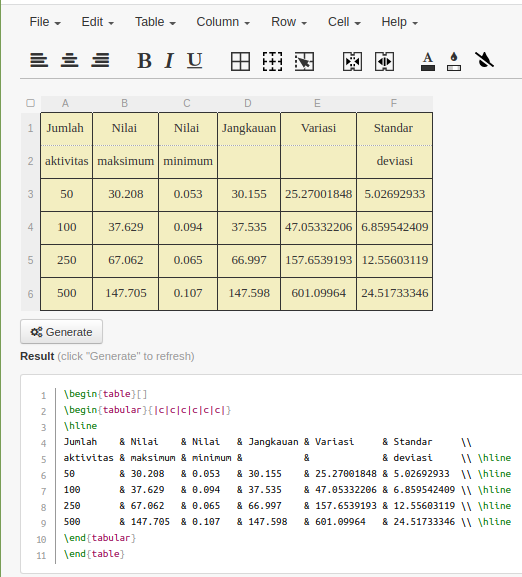
\includegraphics[width=0.5\textwidth]{assets/pics/tablesgenerator-dot-com.png}
	\caption{\textit{User interface} dari \textit{website} https://www.tablesgenerator.com/}
	\label{fig:tablesgenerator}
\end{figure}

Di sisi lain, tabel juga dapat diberi label dan caption seperti pada gambar.
Caption pada tabel terletak pada bagian atas tabel.
Contoh kode yang menyusun suatu tabel sederhana dapat dilihat pada \lst~\ref{code:latexTable}.

\lstinputlisting[language={[latex]tex}, caption=Contoh penggunaan tabel, label=code:latexTable]{assets/codes/tutorial/2-basicTable.tex}

Berikut adalah penjelasan dari \lst~\ref{code:latexTable}:
\begin{itemize}
	\item Baris ke-2: \code{\bslash{}centering} digunakan untuk membuat tabel berada di tengah.
	\item Baris ke-3: \code{\bslash{}caption} digunakan untuk memberikan \f{caption} pada tabel.
	\f{Caption} tersebut diletakkan setelah \code{begin\{tabular\}} agar \f{caption} berada di atas tabel.
	\item Pada baris ke-3, terdapat argumen \code{| l | c r |} yang artinya adalah sebagai berikut:
	\begin{itemize}
		\item \code{|} digunakan untuk membuat garis vertikal pada tabel.
		\item \code{l} digunakan untuk membuat suatu kolom menjadi rata kiri.
		\item \code{c} digunakan untuk membuat suatu kolom menjadi rata tengah.
		\item \code{r} digunakan untuk membuat suatu kolom menjadi rata kanan.
	\end{itemize}
	\item Baris ke-4: \code{\bslash{}label} digunakan untuk memberikan label pada tabel.
	Label ini bisa digunakan di suatu paragraf untuk merujuk pada tabel tersebut,
	dengan cara menuliskan \code{\bslash{}ref\{label\}} pada paragraf.
	\item Baris ke-5: \code{\bslash{}begin\{tabular\}} digunakan untuk memulai pembuatan tabel.
	\item \code{\bslash{}hline} digunakan untuk membuat garis horizontal pada tabel.
	\item \code{\&} digunakan untuk memisahkan antar kolom.
	\item \code{\bslash{}\bslash{}} digunakan untuk memisahkan antar baris.
	\item Baris ke-17 dan 18: Kode untuk mengakhiri pembuatan tabel.
\end{itemize}

Hasil dari \lst~\ref{code:latexTable} akan menjadi \tab~\ref{tab:basic}.

\begin{table}
	\centering
	\caption{Contoh Tabel}
	\label{tab:basic}
	\begin{tabular}{| l | c r |} %
		\hline % garis lurus horizontal
		& kol 1 & kol 2 \\ % baris 1
		\hline %
		baris 1 & 1 & 2 \\ % baris 2
		baris 2 & 3 & 4 \\ % baris 3
		baris 3 & 5 & 6 \\ % baris 4
		baris 4 & 7 & 8 \\ % baris 5
		baris 5 & 9 & 10 \\ % baris 6
		\hline
		\bo{jumlah} & \bo{25} & \bo{30} \\ % baris 7
		\hline
	\end{tabular}
\end{table}



%-----------------------------------------------------------------------------%
\subsection{Tabel Panjang (Lintas Baris)}
\label{sec:latexLongTable}
%-----------------------------------------------------------------------------%
Adapun untuk membuat tabel panjang yang bisa melebihi dari satu halaman,
gunakan perintah \code{\bslash{}begin\{longtable\}} sebagai pengganti \code{\bslash{}begin\{table\}}.
Di dalam \code{longtable} tidak perlu lagi ada \code{\bslash{}begin\{tabular\}}.
Kemudian, tambahkan tanda \code{\bslash{}\bslash{}} setelah baris \code{\bslash{}label\{....\}},
agar tidak menimbulkan error saat menampilkan \f{caption} di bagian atas tabel.
Kemudian, untuk membatasi header yang ingin diulang pada halaman-halaman berikutnya,
gunakan perintah \code{\bslash{}endhead}.
Contoh kode pembuatan tabel pankang dapat dilihat pada \lst~\ref{code:latexLongTable}.

\lstinputlisting[language={[latex]tex}, caption=Contoh penggunaan tabel panjang, label=code:latexLongTable]{assets/codes/tutorial/2-longTable.tex}

Terdapat lima bagian pada sebuah tabel panjang:
\begin{enumerate}
	\item Awalan (\f{header}) di halaman pertama, umumnya disebut sebgai \code{firsthead}.\\
	Pada \lst~\ref{code:latexLongTable}, bagian ini didefinisikan di baris 2 sampai 7.
	Bagian ini diakhiri definisinya dengan perintah \code{\bslash{}endfirsthead}.
	Pada bagian ini, \f{caption} yang digunakan merupakan \f{caption} asli.
	\code{caption} dan \code{label} hanya perlu didefinisikan di bagian awal tabel, di halaman pertama saja.
	Anda juga tetap bisa menggunakan \code{captionsource} apabila dibutuhkan.
	\item Awalan (\f{header}) di halaman berikutnya, umumnya disebut sebagai \code{head}.\\
	Pada \lst~\ref{code:latexLongTable}, bagian ini didefinisikan di baris 8 sampai 12.
	Bagian ini diakhiri definisinya dengan perintah \code{\bslash{}endhead}.
	Terkait penggunaan \f{caption} sambungan:
	\begin{itemize}
		\item Jika Anda menggunakan \code{\bslash{}caption\{\}}, maka untuk menuliskan caption sambungan, gunakan perintah \code{\bslash{}caption[]\{\}}.
		Pada kasus \lst~\ref{code:latexLongTable}, \f{caption} sambungan didefinisikan di baris 8 menggunakan perintah \code{\bslash{}caption[]\{\}}.
		\item Jika Anda menggunakan \code{\bslash{}captionsource\{\}\{\}}, maka untuk menuliskan caption sambungan, gunakan perintah \code{\bslash{}captionsourcecont\{\}\{\}}.
	\end{itemize}
	\item Akhiran (\f{footer}) yang muncul di halaman pertama hingga sebelum terakhir, umumnya disebut sebagai \code{foot}.\\
	Bagian ini diakhiri definisinya dengan perintah \code{\bslash{}endfoot}.
	Pada \lst~\ref{code:latexLongTable}, bagian ini didefinisikan di baris 13 sampai 14.
	Dalam kasus ini, akhiran tabel hanya berupa garis horizontal.
	\item Akhiran (\f{footer}) di halaman terakhir, umumnya disebut sebagai \code{lastfoot}.\\
	Bagian ini diakhiri definisinya dengan perintah \code{\bslash{}endlastfoot}.
	Pada \lst~\ref{code:latexLongTable}, bagian ini didefinisikan di baris 15 sampai 16.
	Dalam kasus ini, akhiran tabel hanya berupa garis horizontal.
	\item Isi dari tabel.
	Pada \lst~\ref{code:latexLongTable}, bagian ini didefinisikan di baris 17 sampai 32.
	Isi dari tabel akan diletakkan di antara awalan tabel (\f{header}) dan akhiran tabel (\f{footer}).
\end{enumerate}

Hasil dari \lst~\ref{code:latexLongTable} akan menjadi \tab~\ref{tab:long}.

\begin{longtable}{| l | c r |}
    \caption{Contoh Tabel Panjang}
    \label{tab:long} \\
    \hline
    & kol 1 & kol 2 \\
    \hline
    \endfirsthead % batas akhir header yang akan muncul di halaman pertama
    \caption[]{Contoh Tabel Panjang (sambungan)} \\
    \hline
    & kol 1 & kol 2 \\
    \hline
    \endhead % batas akhir header yang akan muncul di halaman berikutnya
    \hline
    \endfoot % batas akhir footer yang akan muncul di halaman berikutnya
    \hline
    \endlastfoot % batas akhir footer yang akan muncul di halaman terakhir
    baris 1  & 1 & 2 \\
    baris 2  & 3 & 4 \\
    baris 3  & 5 & 6 \\
    baris 4  & 7 & 8 \\
    baris 5  & 9 & 10 \\
    baris 6  & 11 & 12 \\
    baris 7  & 13 & 14 \\
    baris 8  & 15 & 16 \\
    baris 9  & 17 & 18 \\
    baris 10 & 19 & 20 \\
    baris 11 & 21 & 22 \\
    baris 12 & 23 & 24 \\
    baris 13 & 25 & 26 \\
    baris 14 & 27 & 28 \\
    baris 15 & 29 & 30 \\
    baris 16 & 31 & 32 \\
\end{longtable}


%-----------------------------------------------------------------------------%
\subsection{Menggabungkan (\f{Merge}) Baris atau Kolom}
\label{sec:latexMergeCellsTable}
%-----------------------------------------------------------------------------%
Ada jenis tabel lain yang dapat dibuat dengan \gls{latex}~berikut beberapa diantaranya.
Contoh-contoh ini bersumber dari \url{https://en.wikibooks.org/wiki/LaTeX/Tables}.

\bo{Contoh 1: Menggabungkan Kolom} \\
Contoh penggunaan tabel dengan sel yang melebar ke lebih dari satu kolom dapat dilihat pada \lst~\ref{code:mergeColumnTable}.
Pada contoh ini, sel pada baris 1, kolom 3 dan 4 digabungkan menjadi satu dengan menggunakan perintah \code{\bslash{}multicolumn\{3\}\{c\}\{Week 1\}}.

\lstinputlisting[language={[latex]tex}, caption=Contoh penggunaan tabel dengan sel yang melebar ke lebih dari satu kolom, label=code:mergeColumnTable]{assets/codes/tutorial/2-mergeColumnTable.tex}

Hasil dari \lst~\ref{code:mergeColumnTable} akan menjadi \tab~\ref{tab:rowSpanning}.

\begin{table}
	\centering
	\captionsource{Tabel dengan sel yang melebar ke lebih dari satu kolom}{\url{https://en.wikibooks.org/wiki/LaTeX/Tables}, dengan modifikasi.}
	\label{tab:rowSpanning}
	\begin{tabular}{|l|l|*{6}{c|}}
		% Baris 1
		\hline % buat garis horizontal dari kolom pertama ke kolom terakhir
		No & Name & \multicolumn{3}{|c|}{Week 1} & \multicolumn{3}{|c|}{Week 2} \\
		% Baris 2
		\cline{3-8} % buat garis horizontal dari kolom 3 sampai 8
		& & A & B & C & A & B & C\\
		% Baris 3
		\hline
		1 & Lala & 1 & 2 & 3 & 4 & 5 & 6\\
		% Baris 4
		2 & Lili & 1 & 2 & 3 & 4 & 5 & 6\\
		% Baris 5
		3 & Lulu & 1 & 2 & 3 & 4 & 5 & 6\\
		\hline
	\end{tabular}
\end{table}


\bo{Contoh 2: Menggabungkan Baris} \\
Contoh penggunaan tabel dengan sel yang melebar ke lebih dari satu baris dapat dilihat pada \lst~\ref{code:mergeRowTable}.
Pada contoh ini, sel pada kolom 1, baris 2 dan 3 digabungkan menjadi satu dengan menggunakan perintah \code{\bslash{}multirow\{2\}\{*\}\{Kedua\}}.

\lstinputlisting[language={[latex]tex}, caption=Contoh penggunaan tabel dengan sel yang melebar ke lebih dari satu baris, label=code:mergeRowTable]{assets/codes/tutorial/2-mergeRowTable.tex}

Hasil dari \lst~\ref{code:mergeRowTable} akan menjadi \tab~\ref{tab:columnSpanning}.

\begin{table}
	\centering
	\captionsource{Tabel dengan sel yang melebar ke lebih dari satu baris}{\url{https://en.wikibooks.org/wiki/LaTeX/Tables}, dengan modifikasi.}
	\label{tab:columnSpanning}
	\begin{tabular}{|l|c|l|} % border vertikal ditandai dengan |
        % Baris 1
		\hline % buat garis horizontal dari kolom pertama ke kolom terakhir
		Percobaan & Iterasi & Waktu \\
        % Baris 2
		\hline
		Pertama & 1 & 0.1 sec \\ \hline
        % Baris 3 (kolom 1 melebar 2 baris)
		\multirow{2}{*}{Kedua} & 1 & 0.1 sec \\
        % Baris 4 (kolom 1 dikosongkan karena sudah ditimpa)
		& 3 & 0.15 sec \\
        % Baris 5 (kolom 1 melebar 3 baris)
		\hline
		\multirow{3}{*}{Ketiga} & 1 & 0.09 sec \\
        % Baris 6 (kolom 1 dikosongkan karena sudah ditimpa)
		& 2 & 0.16 sec \\
        % Baris 7 (kolom 1 dikosongkan karena sudah ditimpa)
		& 3 & 0.21 sec \\
		\hline
	\end{tabular}
\end{table}


\bo{Contoh 3: Menggabungkan Baris dan Kolom} \\
Contoh penggunaan tabel dengan sel yang melebar ke lebih dari satu kolom dan baris dapat dilihat pada \lst~\ref{code:mergeBothTable}.

\lstinputlisting[language={[latex]tex}, caption=Contoh penggunaan tabel dengan sel yang melebar ke lebih dari satu kolom dan baris, label=code:mergeBothTable]{assets/codes/tutorial/2-mergeBothTable.tex}

Hasil dari \lst~\ref{code:mergeBothTable} akan menjadi \tab~\ref{tab:mixSpanning}.

\begin{table}
	\centering
	\captionsource{Tabel dengan sel yang melebar ke lebih dari satu kolom dan baris}{\url{https://en.wikibooks.org/wiki/LaTeX/Tables}, dengan modifikasi.}
	\label{tab:mixSpanning}
	\begin{tabular}{|cc|c|c|c|c|} % border vertikal ditandai dengan |, semua kolom rata tengah.
        % 2-row 2-col span (rata tengah), dan 4-col span (rata tengah)
		\hline % buat garis horizontal dari kolom pertama ke kolom terakhir
		\multicolumn{2}{|c|}{\multirow{2}{*}{Element}} & \multicolumn{4}{c|}{Title} \\
        % kelanjutan border untuk 2-row 2-col span, dan 4 kolom biasa
        \cline{3-6} % buat garis horizontal dari kolom 3 sampai 6
		\multicolumn{2}{|c|}{} & A & B & C & D \\
        % 2-row span (rata kiri), dan 5 kolom biasa
        \hline
		\multicolumn{1}{|l|}{\multirow{2}{*}{Type}} & X & 1 & 2 & 3 & 4 \\
        % kelanjutan border untuk 2-row span, dan 5 kolom biasa
        \cline{2-6}
		\multicolumn{1}{|l|}{} & Y & 0.5 & 1.0 & 1.5 & 2.0 \\
        % kelanjutan bordering untuk 2-row span, dan 5 kolom biasa
        % 2-row span (rata kiri), dan 5 kolom biasa
        \hline
		\multicolumn{1}{|l|}{\multirow{2}{*}{Resource}} & I & 10 & 20 & 30 & 40\\
        % kelanjutan border untuk 2-row span, dan 5 kolom biasa
        \cline{2-6}
		\multicolumn{1}{|l|}{} & J & 5 & 10 & 15 & 20 \\
        \hline
	\end{tabular}
\end{table}




%-----------------------------------------------------------------------------%
\section{Membuat Persamaan Matematis}
\label{sec:mathEqu}
%-----------------------------------------------------------------------------%
% v2.2.1: tutorial dipindah dari Bab 3 ke Bab 2
Di \gls{latex}, kita dapat membuat persamaan matematis baik yang terdiri dari satu persamaan maupun lebih dari satu persamaan.
Anda bisa mencoba mengikuti dan memahami contoh kode yang ada di \f{template} ini untuk kebutuhan tugas akhir Anda.
Menggunakan \gls{latex}~juga perlu latihan dan lihai memahami dokumentasi.

%-----------------------------------------------------------------------------%
\subsection{Satu Persamaan}
\label{sec:oneEqu}
%-----------------------------------------------------------------------------%
\noindent \begin{align}\label{equ:garis}
	\cfrac{y - y_{1}}{y_{2} - y_{1}} =
	\cfrac{x - x_{1}}{x_{2} - x_{1}}
\end{align}

\addequtotoc{equ:garis}{Persamaan garis}


\equ~\ref{equ:garis} di atas adalah persamaan garis.
Persamaan tersebut dapat disusun dengan menggunakan perintah \code{\bslash{}align}, seperti yang ditunjukkan pada \lst~\ref{code:singleEquationGaris}.
Penggunaan perintah \code{\bslash{}noindent} sebelum memanggil \f{environment} \code{align} diperlukan agar persamaan yang dicetak tidak tergeser mengikuti indentasi yang umumnya muncul di awal paragraf.
Terdapat beberapa perintah yang digunakan untuk menyusun \equ~\ref{equ:garis}, yaitu:
\begin{itemize}
	\item Perintah \code{\bslash{}cfrac\{\}\{\}} untuk menulis pecahan dalam bentuk vertikal.
	Argumen pertama adalah pembilang (di atas), sedangkan argumen kedua adalah penyebut (di bawah).
	\item Perintah \code{\bslash{}\_\{\}} untuk menulis \f{subscript}.
\end{itemize}

Di luar \f{environment} \code{align}, kita juga bisa menambahkan persamaan tersebut ke daftar persamaan dengan menggunakan perintah \code{\bslash{}addequtotoc\{label\}\{caption\}}.
Perintah \code{\bslash{}label} pada persamaan matematis hanya akan memberikan label,
namun tidak menambahkan ke daftar persamaan.
Perintah \code{\bslash{}addequtotoc} harus ditambahkan di luar \f{environment} \code{align},
karena perintah tersebut harus dijalankan di mode \f{typesetting} teks biasa agar tidak terjadi \f{error}.

\lstinputlisting[language={[latex]tex}, caption=Kode pembuatan \equ~\ref{equ:garis}, label=code:singleEquationGaris]{assets/codes/tutorial/2-singleEquationGaris.tex}

Persamaan bola berikut, yang ditunjukkan oleh \ref{equ:bola}, merupakan contoh lain menyusun sebuah persamaan di \gls{latex}.

\noindent \begin{align}\label{equ:bola}
	\underbrace{|\overline{ab}|}_{\text{pada bola $|\overline{ab}| = r$}}
	= \sqrt[2]{(x_{b} - x_{a})^{2} + (y_{b} - y_{a})^{2} +
		\vert\vert(z_{b} - z_{a})^{2}}
\end{align}

\addequtotoc{equ:bola}{Persamaan bola}


Terdapat beberapa perintah yang digunakan untuk menyusun \equ~\ref{equ:bola}, yaitu:
\begin{itemize}
	\item Perintah \code{\bslash{}sqrt\{\}} untuk menulis akar.
	\item Perintah \code{\bslash{}underbrace\{\}} untuk menulis \f{brace} di bawah suatu ekspresi.
		Biasanya digunakan untuk memberikan anotasi terhadap suatu ekspresi.
	\item Perintah \code{\bslash{}overline\{\}} untuk menulis garis di atas suatu ekspresi.
	\item Perintah \code{\bslash{}text\{\}} untuk menulis teks biasa di dalam persamaan.
	\item Di dalam teks biasa, kita bisa menuliskan kembali sebuah persamaan matematis dengan menambahkan tanda \code{\$} di awal dan di akhir persamaan tersebut.
		Di \gls{latex}, terdapat dua mode \f{typesetting}, yaitu mode teks dan mode matematika.
		Fungsi \code{\$} adalah untuk mengubah mode teks menjadi mode matematika.
	\item Perintah \code{\bslash{}vert} untuk menulis tanda garis vertikal.
\end{itemize}

\lstinputlisting[language={[latex]tex}, caption=Kode pembuatan \equ~\ref{equ:bola}, label=code:singleEquationBola]{assets/codes/tutorial/2-singleEquationBola.tex}

Suatu persamaan yang dibuat menggunakan \f{environment} \code{align} akan secara otomatis memiliki indeks (nomor) dari persamaan.
Perintah \code{align} ini juga dapat digunakan untuk menulis lebih dari satu persamaan.


%-----------------------------------------------------------------------------%
\subsection{Lebih dari Satu Persamaan}
\label{sec:multiEqu}
%-----------------------------------------------------------------------------%
\equ~\ref{equ:matriks} adalah contoh persamaan matriks yang dibuat menggunakan \gls{latex}.

\noindent \begin{align}\label{equ:matriks}
	|\overline{a} * \overline{b}| &= |\overline{a}| |\overline{b}| \sin\theta
	\\[0.2cm]
	\overline{a} * \overline{b} &=
	\begin{array}{| c c c |}
		\hat{i} & x_{1} & x_{2} \\
		\hat{j} & y_{1} & y_{2} \\
		\hat{k} & z_{1} & z_{2} \\
	\end{array} \nonumber \\[0.2cm]
	&= \hat{i} \,
	\begin{array}{ | c c | }
		y_{1} & y_{2} \\
		z_{1} & z_{2} \\
	\end{array}
	+ \hat{j} \,
	\begin{array}{ | c c | }
		z_{1} & z_{2} \\
		x_{1} & x_{2} \\
	\end{array}
	+ \hat{k} \,
	\begin{array}{ | c c | }
		x_{1} & x_{2} \\
		y_{1} & y_{2} \\
	\end{array}
	\nonumber
\end{align}

\addequtotoc{equ:matriks}{Persamaan matriks}


Pada \equ~\ref{equ:matriks} dapat dilihat beberapa baris persamaan menjadi satu bagian dari persamaan tersebut.
Kode untuk menyusun kumpulan persamaan di \equ~\ref{equ:matriks} dapat dilihat pada \lst~\ref{code:multiEquationAsOne}.
Eksekusi perintah \code{\bslash{}addequtotoc\{label\}\{caption\}} juga cukup dilakukan sekali saja.

\lstinputlisting[language={[latex]tex}, caption=Kode pembuatan \equ~\ref{equ:matriks}, label=code:multiEquationAsOne]{assets/codes/tutorial/2-multiEquationAsOne.tex}

Terdapat beberapa perintah yang digunakan untuk menyusun \equ~\ref{equ:matriks}, yaitu:
\begin{itemize}
	\item Perintah \code{\bslash{}begin\{array\}} dan \code{\bslash{}end\{array\}} untuk membuat matriks.
	Cara kerja \f{environment} \code{array} sama dengan \f{environment} \code{tabular} yang digunakan untuk membuat tabel.
	\item Perintah \code{\bslash{}sin} untuk menulis fungsi sinus.
	\item Perintah \code{\bslash{}theta} untuk menulis simbol theta ($\theta$).
	\item Perintah \code{\bslash{}hat\{\}} untuk menulis tanda aksen \f{hat} (\^{}) di atas suatu huruf.
\end{itemize}

Sedangkan dibawah ini dapat dilihat bahwa dengan cara yang sama, \equ~
\ref{equ:integral}, \ref{equ:limit}, dan \ref{equ:eksponen} memiliki nomor
persamaannya masing-masing.

\noindent \begin{align}
	\label{equ:integral}
	\int_{a}^{b} f(x)\, dx + \int_{b}^{c} f(x) \, dx = \int_{a}^{c} f(x) \, dx \\
	\label{equ:limit}
	\lim_{x \to \infty} \frac{f(x)}{g(x)} = 0 \hspace{1cm}
	\text{jika pangkat $f(x)$ $<$ pangkat $g(x)$} \\
	\label{equ:eksponen}
	a^{m^{a \, ^{n}\log b }} = b^{\frac{m}{n}}
\end{align}

\addequtotoc{equ:integral}{Persamaan integral}
\addequtotoc{equ:limit}{Persamaan limit}
\addequtotoc{equ:eksponen}{Persamaan eksponen dan logaritma}


Kode yang menyusun \equ~\ref{equ:integral}, \ref{equ:limit}, dan \ref{equ:eksponen} dapat dilihat pada \lst~\ref{code:multiEquationAsSeparate}.
Perbedaan penyusunan tiga argumen tersebut dibandingkan dengan \equ~\ref{equ:matriks} adalah penggunaan \f{label} pada setiap persamaan.
Pada \equ~\ref{equ:matriks}, \f{label} diletakkan pada bagian awal persamaan pertama, sehingga hanya satu \f{label} yang digunakan.
Pada \equ~\ref{equ:integral}, \ref{equ:limit}, dan \ref{equ:eksponen}, \f{label} diletakkan pada awal setiap persamaan, sehingga setiap persamaan memiliki \f{label} masing-masing.
Selain itu, jika ingin memasukkan setiap persamaan secara terpisah ke Daftar Persamaan,
eksekusi perintah \code{\bslash{}addequtotoc\{label\}\{caption\}} juga harus dilakukan terpisah untuk setiap persamaan.

\lstinputlisting[language={[latex]tex}, caption={Kode pembuatan \equ~\ref{equ:integral}, \ref{equ:limit}, dan \ref{equ:eksponen}}, label=code:multiEquationAsSeparate]{assets/codes/tutorial/2-multiEquationAsSeparate.tex}

Terdapat beberapa perintah yang digunakan untuk menyusun \equ~\ref{equ:integral}, \ref{equ:limit}, dan \ref{equ:eksponen}, yaitu:
\begin{itemize}
	\item Perintah \code{\bslash{}int} untuk menulis simbol integral.
	Untuk batas bawah dan batas atas integral, bisa dituliskan dengan menggunakan perintah \f{subscript} dan \f{superscript}.
	\item Perintah \code{\bslash{}lim} untuk menulis simbol limit.
	\item Perintah \code{\bslash{}to} untuk menulis panah ke kanan.
	\item Perintah \code{\bslash{}infty} untuk menulis simbol tak hingga.
	\item Perintah \code{\bslash{}log} untuk menulis fungsi logaritma.
	Pangkat basis logaritma dituliskan dengan menggunakan perintah \f{superscript} sebelum perintah \code{\bslash{}log}.
\end{itemize}


%-----------------------------------------------------------------------------%
\section{Menambahkan Kode Program}
\label{sec:codeListing}
% Hal baru di template 2017
%-----------------------------------------------------------------------------%
% v2.2.1: tutorial dipindah dari Bab 3 ke Bab 2
Pada \gls{latex}, kode program seringkali disebut \f{listing}.
\f{Syntax highlighting} kini sudah bisa dilakukan secara otomatis oleh \f{library} yang ada di \gls{latex}.
Sudah tidak perlu lagi membuat skrip manual untuk menambahkan \f{syntax highlighting} sendiri.
\lst~\ref{code:java} adalah contoh kode program (\f{listing}) Java yang dicetak oleh \gls{latex}.

\lstinputlisting[language=Java, caption=Kode sampel Java yang cukup panjang, label=code:java]{assets/codes/2-sample.java}

Sintaks untuk memasukkan kode program ke dalam dokumen \gls{latex}~adalah sebagai berikut:

\begin{lstlisting}[language={[latex]tex}, caption=Meng]
\lstinputlisting[language=Java, caption=Kode sampel Java yang cukup panjang, label=code:java]{assets/codes/2-sample.java}
\end{lstlisting}

Terdapat tiga argumen yang digunakan pada perintah \code{\bslash{}lstinputlisting}:
\begin{itemize}
	\item \code{language} digunakan untuk menentukan bahasa pemrograman yang digunakan.
	Untuk menggunakan suatu dialek bahasa pemrograman yang berbeda dari \f{default},
	misalkan versi Python3 dari Python,
	gunakan perintah \code{language=\{[3]Python\}}.
	\item \code{caption} digunakan untuk memberikan \f{caption} pada kode program.
	Argumen ini sifatnya opsional, jika ada, maka \f{caption} akan ditampilkan di bawah kode program.
	Jika argumen ini tidak ada, maka \f{caption} tidak akan ditampilkan dan kode tidak bisa masuk ke daftar kode program.
	\item \code{label} digunakan untuk memberikan label pada kode program untuk rujukan di dalam dokumen (\f{cross-reference}).
	Argumen ini tidak boleh didefinisikan jika argumen \code{caption} tidak didefinisikan.
\end{itemize}

Terdapat empat kelompok bahasa pemrograman (dan dialek) yang didukung oleh implementasi \code{listings} pada \f{template} ini, yaitu:

\begin{itemize}
	\item \bo{Bahasa pemrograman yang didukung secara \f{default} oleh \code{listings}} (menurut \cite{latex:source_code_listings}): \\
		\code{ABAP}, \code{ACSL}, \code{Ada}, \code{Algol}, \code{Ant}, \code{Awk}, \code{bash}, \code{Basic}, \code{C++}, \code{C}, \code{Caml},
		\code{Clean}, \code{Cobol}, \code{Comal}, \code{command.com} (Windows Batch), \code{csh}, \code{Delphi}, \code{Eiffel}, \code{Elan},
		\code{erlang}, \code{Euphoria}, \code{Fortran}, \code{GCL}, \code{Go} (golang), \code{Gnuplot}, \code{Haskell}, \code{HTML}, \code{IDL},
		\code{inform}, \code{Java}, \code{JVMIS}, \code{ksh}, \code{Lisp}, \code{Logo}, \code{Lua}, \code{make}, \code{Mathematica}, \code{Matlab},
		\code{Mercury}, \code{MetaPost}, \code{Miranda}, \code{Mizar}, \code{ML}, \code{Modelica}, \code{Modula-2}, \code{MuPAD}, \code{NASTRAN},
		\code{Oberon-2}, \code{OCL}, \code{Octave}, \code{Oz}, \code{Pascal}, \code{Perl}, \code{PHP}, \code{PL/I}, \code{Plasm}, \code{POV},
		\code{Prolog}, \code{Promela}, \code{PSTricks}, \code{Python}, \code{R}, \code{Reduce}, \code{Rexx}, \code{RSL}, \code{Ruby}, \code{S},
		\code{SAS}, \code{Scilab}, \code{sh}, \code{SHELXL}, \code{Simula}, \code{SQL}, \code{tcl}, \code{TeX}, \code{VBScript}, \code{Verilog},
		\code{VHDL}, \code{VRML}, \code{XML}, dan \code{XSLT}.
	\item \bo{Dialek yang didukung secara \f{default} oleh \code{listings}} (menurut \cite{latex:source_code_listings}, diambil beberapa contoh):
		\begin{itemize}
			\item Dialek Assembly: \code{[Motorola68k]\{Assembler\}}, \code{[x86masm]\{Assembler\}},
			\item Dialek Awk: \code{[gnu]\{Awk\}} (GNU Awk), \code{[POSIX]\{Awk\}},
			\item Dialek C: \code{[ANSI]\{C\}} (default), \code{[Handel]\{C\}}, \code{[Objective]\{C\}} (Objective-C), \code{[Sharp]\{C\}} (C\#),
			\item Dialek Caml: \code{[Objective]\{Caml\}} (OCaml), \code{[light]\{Caml\}} (default),
			\item Dialek C++: \code{[11]\{C++\}}, \code{[ANSI]\{C++\}}, \code{[GNU]\{C++\}}, \code{[Visual]\{C++\}} (Visual C++),
				\code{[ISO]\{C++\}} (default),
			\item Dialek Java: \code{[]\{Java\}} (default), \code{[AspectJ]\{Java\}},
			\item Dialek Pascal: \code{[Borland6]\{Pascal\}}, \code{[XSC]\{Pascal\}}, \code{[Standard]\{Pascal\}} (default),
			\item Dialek Python: \code{[2]\{Python\}} (default, Python 2), \code{[3]\{Python\}} (Python 3),
			\item Dialek TeX: \code{[LaTeX]\{TeX\}} (LaTeX), \code{[AlLaTeX]\{TeX\}}, \code{[plain]\{TeX\}} (plain TeX, default),
			\item Dialek tcl: \code{[]\{Tcl\}} (default Tcl), \code{[tk]\{Tcl\}} (Tcl/Tk).
		\end{itemize}
	\item \bo{Bahasa pemrograman yang ditambahkan pada \f{template} ini}: \\
		\code{ABS}, \code{Acceleo}, \code{Batch}, \code{Clojure}, \code{CSS}, \code{D}, \code{Dart}, \code{Docker}, \code{F\#} (FSharp),
		\code{GDScript} (Godot), \code{GLSL}, \code{Groovy}, \code{HLSL}, \code{JavaScript}, \code{Julia}, \code{Kotlin}, \code{Markdown},
		\code{PowerShell}, \code{Rust}, \code{Scala}, \code{Scheme}, \code{Solidity}, \code{Swift}, \code{TOML}, \code{TypeScript}, dan \code{YAML}.
	\item \bo{Dialek yang ditambahkan pada \f{template} ini}:
		\begin{itemize}
			\item Dialek HTML: \code{[v5]\{HTML\}} (HTML5),
			\item Dialek Java: \code{[v9]\{Java\}} (Java 9 Modules), \code{[ContextJ]\{Java\}}, \code{[DeltaJ]\{Java\}}, dan \code{[FOP]\{Java\}}.
		\end{itemize}
\end{itemize}

Berikut adalah contoh penggunaan dialek bahasa pemrograman dalam menuliskan kode program.
Dalam kasus ini, \lst~\ref{code:python2} merupakan kode Python versi 2.
Sedangkan, \lst~\ref{code:python3} merupakan kode Python versi 3.
Perbedaan antara kedua versi tersebut cukup signifikan, salah satunya adalah pada perintah \code{print}.
Pada Python 2, perintah \code{print} tidak memerlukan tanda kurung karena merupakan sebuah \f{keyword},
sedangkan pada Python 3, perintah \code{print} memerlukan tanda kurung karena merupakan sebuah \f{function}.

\lstinputlisting[language=Python, caption=Kode Python 2, label=code:python2]{assets/codes/2-sample-python2.py}

\lstinputlisting[language={[3]Python}, caption=Kode Python 3, label=code:python3]{assets/codes/2-sample-python3.py}

Kode yang mencetak \lst~\ref{code:python2} dan \lst~\ref{code:python3} adalah sebagai berikut:

\begin{lstlisting}[language={[latex]tex}]
\lstinputlisting[language=Python, caption=Kode Python 2, label=code:python2]{assets/codes/2-sample-python2.py}
\lstinputlisting[language={[3]Python}, caption=Kode Python 3, label=code:python3]{assets/codes/2-sample-python3.py}
\end{lstlisting}

Secara \f{default}, dialek yang digunakan untuk Python pada \f{library} \code{listings} adalah Python 2.
Sehingga untuk mencetak kode Python 3, perlu digunakan dialek Python 3 (\code{\{[3]Python\}}).

Kode program yang dicetak oleh \gls{latex} bersifat \f{auto-wrapped}.
Jika suatu baris kode program melebihi batas lebar halaman,
maka kode program tersebut akan dipindahkan ke baris berikutnya.
\f{Auto-wrapped} ini berguna agar Anda tidak perlu memberikan \f{line break} manual pada kode Anda,
Anda bisa menyampaikan kode program Anda apa adanya.

\bo{Catatan}: Jangan lupa untuk menjelaskan kode melalui paragraf,
terutama pada bagian-bagian yang perlu penjelasan lebih.
Setiap kode perlu dijelaskan, kalau bisa rujuk ke setiap baris, karena belum tentu pembaca mau membaca kode Anda.
Tetapi, pembaca tetap perlu mengetahui ide di balik kode yang Anda buat, dan mengapa kode tersebut dibuat.



%-----------------------------------------------------------------------------%
\section{Keterkaitan Teori Dengan Penelitian}
\label{sec:keterkaitan}
%-----------------------------------------------------------------------------%
\todo{
	Ada baiknya setelah menjelaskan teori-teori, Anda menjelaskan apa kaitan teori tersebut dengan penelitian Anda.
	Hal ini tentunya membantu pembaca dalam memahami bahwa teori yang Anda paparkan memang penting untuk memahami penelitian Anda nantinya.
}

\begin{figure}
	\centering
	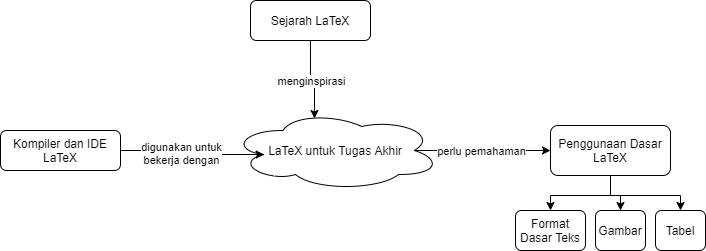
\includegraphics[width=\textwidth]{assets/pics/research_concept_map.png}
	\caption{Keterkaitan konsep hasil studi literatur terhadap penelitian}
	\label{fig:research_concept_map}
\end{figure}

\todo{
	Jelaskan \pic~\ref{fig:research_concept_map} di sini.
	Setiap gambar pada tugas akhir butuh penjelasan.
	Gambar hadir untuk mempermudah membaca memahami konteks, tetapi tidak bisa berdiri sendiri tanpa penjelasan.
}
